%必要事項(全体)
%内容の改善
%図の改善
%現在形と過去形のチェック
%表現の統一
%改ページのチェック
%載せた論文に目を通す
%参考文献の調整

%文字の大きさ、紙の大きさ、ドライバ、エンジン、文書クラス
\documentclass[10pt,a4paper,dvipdfmx,uplatex]{jsreport}

%ページ番号の出力
\pagestyle{plain}

%画像
\usepackage{graphicx}
%位置指定
\usepackage{float}
%ハイパーリンク
\usepackage{hyperref,pxjahyper}
%数式
\usepackage{amsmath,amssymb}
%アルゴリズム
\usepackage[boxed,figure]{algorithm2e}
%文字色
\usepackage{color}
%コメントアウト
\usepackage{comment}
%かっこいい表
\usepackage{booktabs}
%タイトルの調整
\usepackage{titlesec}
%括弧の設定
\usepackage{interval}
%IfAppendix
\usepackage{apptools}
%参照の変更
\usepackage{prettyref}
%目次の設定
\usepackage{tocloft}
\usepackage{etoolbox}
%図の設定
\usepackage[subrefformat=parens]{subcaption}

%ハイパーリンクの設定

%タイトルの番号付けの設定
\setcounter{secnumdepth}{3}

%各種タイトルの設定
\titleformat{\chapter}[hang]{\Huge\bfseries}{\IfAppendix{\appendixname\Alph{chapter}}{第\thechapter~章}}{1zw}{}{}
\titlespacing*{\chapter}{0pt}{0pt}{50pt}
\titleformat*{\section}{\LARGE\bfseries}
\titlespacing{\section}{0pt}{20pt}{15pt}
\titleformat*{\subsection}{\Large\bfseries}
\titlespacing{\subsection}{0pt}{15pt}{10pt}
\titleformat*{\subsubsection}{\large\bfseries}
\titlespacing{\subsubsection}{0pt}{10pt}{6pt}

%目次の設定
\renewcommand{\cfttoctitlefont}{\Huge\bfseries}
\renewcommand{\cftchapfont}{\normalsize\bfseries}
\setlength{\cftchapnumwidth}{4em}
\renewcommand{\cftchapleader}{\cftdotfill{\cftchapdotsep}}
\renewcommand{\cftchapdotsep}{\cftdotsep}

%図目次の設定
\renewcommand{\cftloftitlefont}{\Huge\bfseries}
\renewcommand{\cftfigpresnum}{図~}
\setlength{\cftbeforefigskip}{0pt}
\cftsetindents{figure}{1.5em}{5em}
%図目次にchapterを加える
\preto\figure{
  \ifnum\value{figure}=0
  \phantomsection
  \addtocontents{lof}{
  \begin{flushleft}
    \IfAppendix{\normalsize\bfseries{\appendixname\Alph{chapter}}}{\normalsize\bfseries{第\thechapter~章}}
  \end{flushleft}
  \par
  \vspace{-7.5pt}
  }
  \fi
}

%開き括弧の設定
\intervalconfig{soft open fences}

%align用の箱の作成
\newlength{\alignwidth}
% #1:左側のテキスト、#2:右側のテキスト
\newcommand{\algalign}[2]{\makebox[\alignwidth][l]{#1}~#2}

%参照の変更(prettyref)
\newrefformat{sec}{\ref{#1}節}
\newrefformat{fig}{図\ref{#1}}
\newrefformat{tab}{表\ref{#1}}
\newrefformat{eq}{式\ref{#1}}
\newrefformat{cha}{第\ref{#1}~章}
\newrefformat{app}{\appendixname\ref{#1}}

%argmaxとargminのコマンド
\newcommand{\argmax}{\mathop{\mathrm{arg~max~}}\limits}
\newcommand{\argmin}{\mathop{\mathrm{arg~min~}}\limits}

\begin{document}

%タイトル
\begin{titlepage}
\begin{center}
\vspace*{160truept}
{\huge ニューラルネットワークによる}\\
\vspace{10truept}
{\huge 音楽の自動変換}\\
\vspace{200truept}
{\Large 教養学部後期課程学際科学科総合情報学コース}\\
\vspace{10truept}
{\Large 陶山大輝}\\
\vspace{10truept}
{\Large 学籍番号:08-192021}\\
\vspace{10truept}
{\Large 指導教官:金子知適准教授}\\  
\end{center}
\end{titlepage}

%目次
\setcounter{tocdepth}{2}
\tableofcontents
\phantomsection
\addtocontents{toc}{~\hfill\textbf{Page}\par}
\clearpage

%図目次
\listoffigures
\phantomsection
\addtocontents{lof}{~\hfill\textbf{Page}\par}
\clearpage

%はじめに
\chapter{はじめに}

音楽は世界中で楽しまれている。音楽の作成方法には様々なものがあり、既存の曲をアレンジして新しい曲を作成するRemixと呼ばれる方法がある。しかし、Remixは画面上で音を操作するソフトウェアアプリケーション~(DAW)~を用いるのが一般的である。初心者がDAWを使用するのは難しいため、コンピュータプログラムによる補助が役に立つと考えられる。本研究では、Remixの代表的な方法の一つである音色の変換に着目し、プログラムによる変換手法を提案する。

音色の変換を行うためには、ある楽器の音を異なる楽器の音へ変換する技術が必要である。そこで、本研究ではPix2pix~\cite{pix2pix}を音色の変換に応用した。Pix2pixはニューラルネットワークにより自然な画像を生成する手法であるGenerative~Adversarial~Networks~(GAN)~\cite{GAN}を用いて画像のスタイル変換を行う手法である。

本研究では、ギターの単音をハープの単音に提案手法を用いて変換する実験を行った。その結果、音の大きさが変わることなどの問題はあったものの、ほとんどの音で音程を維持したまま音色の変換を行うことに成功した。また、データセットの一部の音のみで学習を行った場合でも、ほとんどの音で音程を維持したまま変換を行うことができた。

なお、本論文では、音は楽譜作成ソフトのMuseScore\footnote{\url{https://musescore.org/}}により作成し、音波の画像は音声編集ソフトのAudacity\footnote{\url{https://www.audacityteam.org/}}により作成した。

\begin{comment}
%ここから
%短期vs長期
%長期は生成しておいて短期は後から
%音楽の研究の例は関連研究に
既存研究の軽い紹介…。GAN,Pix2pix…。音楽の変換の研究(Hukebox,スペクトログラム,MIDI)…。この手法では…。音色の変換のみを扱うことで短期的な構造のみに着目できる点で他の音楽生成の研究よりも計算時間を削減できると期待される。
~\cite{Jukebox}
\end{comment}

%背景:音楽
\chapter{背景:音楽}

本章では、本論文での音の定義を行った後に、音楽の特徴量抽出の方法を紹介する。

\section{音の定義}

音とは、弾性体中を伝播する弾性波により起こされる音波が聴覚により感じられるもののことである。また、音は騒音と楽音の大きく二つに分けることができる。騒音とは不規則な振動の音波による音のことであり、楽音とは周期生のある音波による音のことである。本論文では、楽音のことを音と呼ぶ。

音は長さ、大きさ、高さ、音色の四要素から成り立ち、人間はこれらの要素を知覚することができる。また、図\ref{fig:gakuon}は音の四要素について簡単に示した図である。

\begin{figure}[b]
\begin{center}
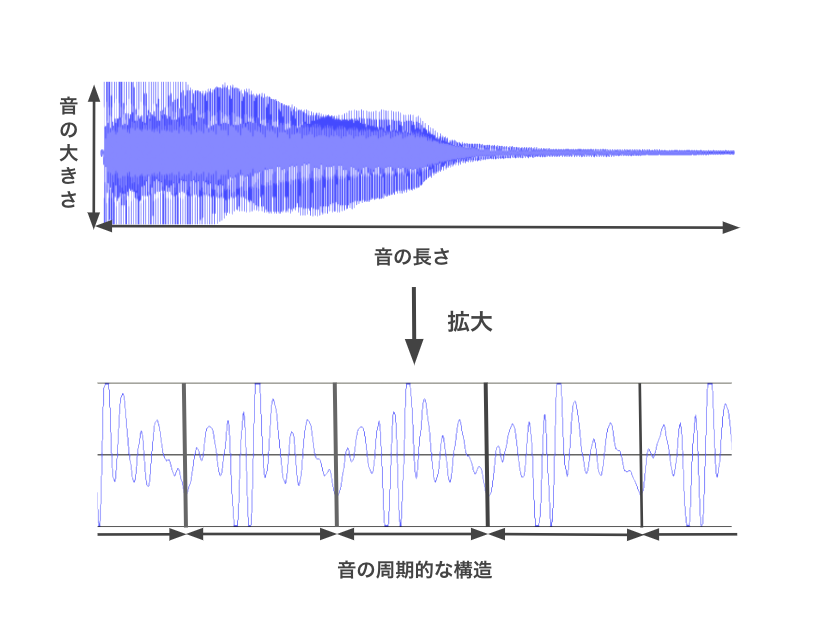
\includegraphics[width=0.6\hsize]{figure/gakuon.png}
\caption{音の四要素}
\label{fig:gakuon}
\end{center}
\end{figure}

\subsection{音の長さ}

音の長さは図\ref{fig:gakuon}のように音波の時間の長さにより決まる。一般に、音の長さは楽譜上での時間の長さ~(音価)~により決まるが、本論文では音波の時間の長さにより決まるものとする。

\subsection{音の大きさ}

音の大きさは図\ref{fig:gakuon}のように音波の振幅により決まる。また、人間には振幅の大きい音は大きく、振幅の小さい音は小さく知覚される。

\subsection{音の高さ}

音の高さは音波の周波数により決まる。つまり、図\ref{fig:gakuon}のような音の周期的な構造の長さにより決まる。また、人間には周波数の高い音は高く、周波数の低い音は低く知覚さる。そして、複数の周波数の音波が音に含まれる場合は最も低い周波数成分の音波~(基音)~を音の高さとして知覚する。

国際の音名表記では、C,D,E,F,G,A,Bのセットを西洋音楽の七音音階におけるオクターブとして定める。さらに、それぞれのオクターブに番号を振り、440~Hzの音をA4と定めることで、任意の半音の絶対的な表記を可能にしている。また、国際の音名表記では半音よりさらに細かい音~(微分音)~を表すことはできないが、本論文では扱わない。

\subsection{音の音色}

音の長さと高さと大きさが同じであっても異なった音として人間には知覚されることがある。この違いを音色と呼ぶ。また、音色は図\ref{fig:gakuon}のような音の周期的な構造の形により決まる。

\begin{figure}[b]
\begin{center}
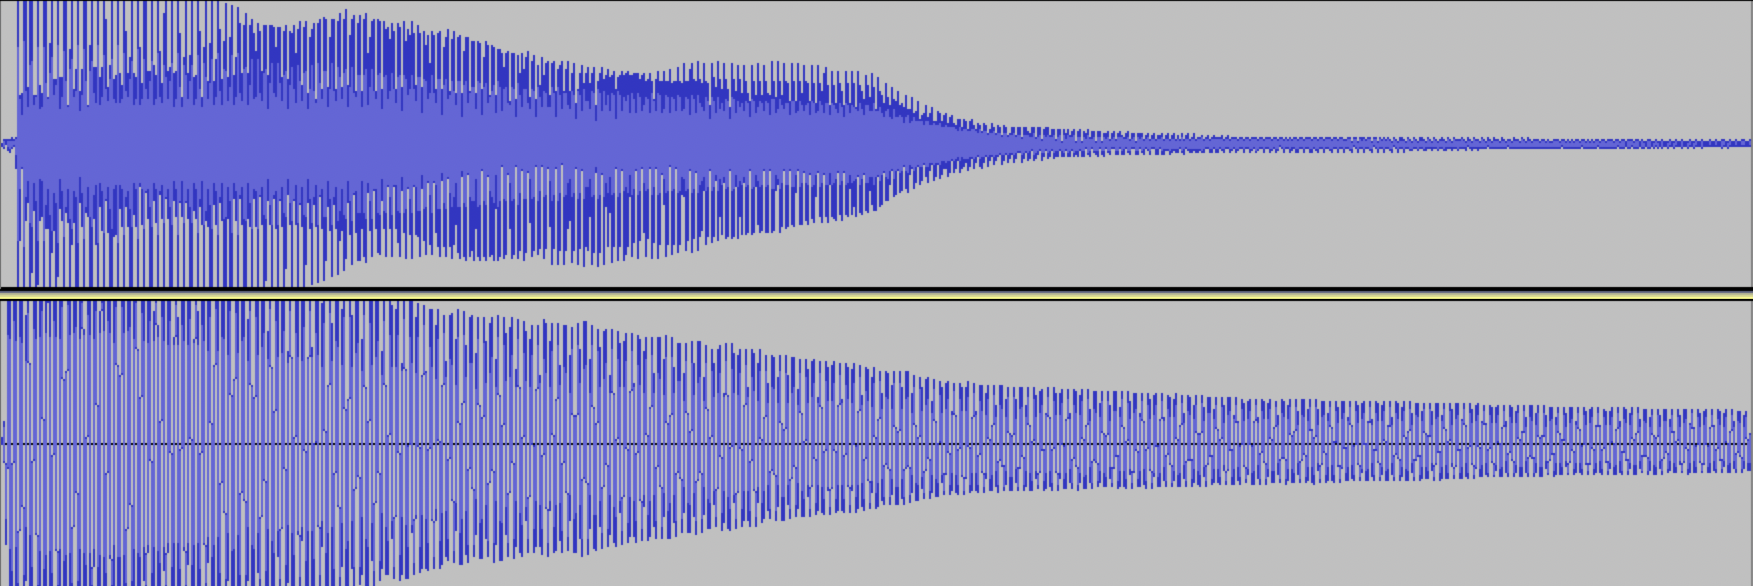
\includegraphics[width=\hsize]{figure/c4_guitar_harp.png}
\caption{ギターとハープの音色}
\label{fig:guitar_harp_comp}
\end{center}
\end{figure}

ここで、長さと高さと大きさが同じギターとハープの音波を図\ref{fig:guitar_harp_comp}に示す。これらの音は波形が異なるので、その音色も異なる。また、音色の異なる音どうしは基音よりも高い音~(上音)~の組み合わせが異なるため、このような波形の違いが生まれる。

\section{音楽の特徴}

%以下の自分の考えと融合させる
\begin{comment}
\section{展望}

一般に、音楽で特定の音色への変換を行うことは難しいが、次の三つの要素に分解することで単音での音色の変換を音楽へと適用することが可能であると考えられる。また、三つの要素とは、楽器の重ね合わせ、音の重ね合わせ、時間方向の音の繋ぎ方であり、それぞれについて具体的に以下で説明をする。

\subsection{楽器の重ね合わせ}
    
音楽はそれぞれの楽器により奏でられた音の重ね合わせになっている。楽器ごとに音色は異なるので楽器ごとの音波に分解して音色変換を行う~(音源分離)~が必要であると考えられる。なお、楽曲の作成時に楽器ごとに分離したデータ~(パラデータ)~で保存しておけば、音源分離を行わずに直接楽器ごとの音波を利用できる。

\subsection{音の重ね合わせ}

ある単位時間の音に注目した時、楽器ごとの音波に分解してもその単位時間で異なった高さや大きさの音の重ね合わせになっていることがある。この場合は、今回の提案手法で用意したデータセット以外に和音のデータセットも加えて学習させることで表現可能であると考えられる。

\subsection{音の繋ぎ方}

%他の工夫があるかも

楽器ごとの音波に分解し単位時間の音が表現できた時、時間方向に音を繋ぐ必要がある。時間方向については先程定めた単位時間で区切って順に変換していくことで可能であると 考えている。また、区切るのみでの変換が難しい場合は自己回帰モデルを取り入れるなどの工夫が必要であると考えている。
\end{comment}

音楽をニューラルネットワークにて扱う場合、音楽特有の特徴量抽出が必要である。また、音楽の特徴には、主観的な問題とタイムスケールの問題がある。

\subsection{音楽の主観性}

まず、主観性について。例えば、音楽のジャンルの分け方はかなり主観に依存する。それに対し、ピッチやテンポは主観性が弱い(が、曖昧でもある)。ディープラーニングはこれらの二つの問題に対してある程度対応できている。主観さの裏にある論理を解明しない限りは、人間の手で特徴量を設定するのは難しい。従って、データ駆動でend-to-endな学習を利用することができる。さらに、新たな洞察を得ることもできる。例えば、異なる音楽間の関係性。また、よく知られた論理があればネットワーク構築にも役立つ。

\subsection{音楽の時間方向のスケール}

次にタイムスケールについて、考慮すべき時間のスケール。例えば、テンポや音の高さは音楽全体では変化するものの短い時間で見れば静的である。このような場合は時間のスケールは長いと言える(時間不変性の問題)。それに対し、音色は短いスケールのタイムフレームであっても変わりうる。従って、このような場合は時間のスケールは短い(時間可変性の問題)。

このように、それぞれの特徴が異なった主観性やタイムスケールを持つので、対処法が変わってしまう。

\section{音楽の表現}
\label{sec:preprocess}

ニューラルネットワークで扱うために音の表現を工夫する必要がある。ニューラルネットワークの学習を行う場合は音楽を音響信号としてサンプリングした際の一次元データではなく、何らかの加工を施した二次元データを用いることが多い。また、この二次元の軸は時間と周波数であることが多い。



\subsection{音響信号}

\subsection{STFT}

\subsection{メルスペクトログラム}

\subsection{CQT}

\subsection{クロマグラム}

\subsection{DDSP}

%音声処理勉強してここに載せる(大幅な改変)
%いいやつを見つけた

%以下の流れ

%まず基本的なこと

%既存研究でもこんな感じ

%それぞれに特徴があるけど…

\begin{comment}
本章では、主要な音声処理の方法を紹介する。

以下の単語は説明

サンプリング周波数] デジタル信号の1秒あたりの標本化の回数

サンプリング数] 音波のデジタル信号の標本化の合計の回数のこと

量子化ビット数] デジタル信号の細かさを表現するビット数のこと

チャンネル数] モノラルな音声出力の総数のこと

%短期vs長期
%長期は生成しておいて短期は後から
%音楽の研究の例はをどこかに
既存研究の軽い紹介…。GAN,Pix2pix…。音楽の変換の研究(Hukebox,スペクトログラム,MIDI)…。この手法では…。音色の変換のみを扱うことで短期的な構造のみに着目できる点で他の音楽生成の研究よりも計算時間を削減できると期待される。
\end{comment}

%背景:ニューラルネットワーク
\section{ニューラルネットワーク}
ニューラルネットワークとはニューロンとニューロン間のシナプスによる結合で形成される脳のネットワークを模した数理モデルである。入力層と出力層を持ち、シナプスの結合強度を変化させることで問題に最適なネットワークを構成することを目標とする。\par
また、入力層と出力層の間に隠れ層を加えて多層にし層間に活性化関数を用いて非線形分離を行うことで、複雑なネットワークを作ることができる。さらに、任意の活性化関数が微分可能であれば、誤差逆伝播法により損失関数を高速に求めることができる。\par


\section{ディープラーニング}

ディープラーニングとは層をより深くしたニューラルネットワークを用いた機械学習の手法である。多大な計算資源を必要とするが、GPUを含む計算機の性能の向上により実用的な手法となった。\par
また、層を増やすと勾配の減衰による勾配消失や訓練データへの最適化による過学習などの問題が発生するが、前者の場合は活性化関数にReLU関数を用い後者の場合は汎化性能を測定することで避けることができる。\par

%以下、abst,intro,method,しか読んでないものがほとんど

\section{GAN}

GAN(敵対的生成モデル)とは生成モデルと識別モデルが競合して学習を行うディープラーニングのモデルである。生成モデルは訓練データの分布を捉えようとし、識別モデルは訓練データである確率を推定する。\par
具体的には、訓練データの分布を$p_{data}$,生成モデルの入力となるノイズの分布を$p_z$,ノイズを元にデータを生成する関数を$G$,生成モデルのデータではなく訓練データである確率を返す関数を$D$とした時、下記の式を生成モデルは最小化し識別モデルは最大化をすることを目標として学習を行う\cite{GAN}。

$$
\mathbb{E}_{\boldsymbol{x} \sim p_{\text {data }}(\boldsymbol{x})}[\log D(\boldsymbol{x})]+\mathbb{E}_{\boldsymbol{z} \sim p_{\boldsymbol{z}}}(\boldsymbol{z})[\log (1-D(G(\boldsymbol{z})))]
$$

\section{CGAN}

CGAN(条件付き敵対的生成モデル)とは条件付きのGANである。具体的には$y$という条件下で下記の式を生成モデルは最小化し識別モデルは最大化をすることを目標として学習を行う\cite{CGAN}。\par
原著論文では訓練時にMNISTの数字のラベルを条件として与えることで特定の数字のラベルの画像を生成するモデルを実装している。

$$
\mathbb{E}_{\boldsymbol{x} \sim p_{\text {data }}(\boldsymbol{x})}[\log D(\boldsymbol{x} \mid \boldsymbol{y})]+\mathbb{E}_{\boldsymbol{z} \sim p_{z}(\boldsymbol{z})}[\log (1-D(G(\boldsymbol{z} \mid \boldsymbol{y})))]
$$

\section{pix2pix}

pix2pixとはある条件下で画像間の変換を行うGANである。先程のCGANを元にU-NetとPatachGANを組み合わせたネットワークになっている。\textcolor{red}{U-netとは…,PatachGANとは…。(ここは後々調べて書く)}\par
具体的には、画像$x$を条件として(3)式を生成モデルは最小化し識別モデルは最大化をすることを目標として学習を行う\cite{pix2pix}。

$$
\mathcal{L}_{cGAN}(G, D)=\mathbb{E}_{x, y}[\log D(x, y)]+\mathbb{E}_{x, z}[\log (1-D(x, G(x, z)))] \eqno(1)
$$
$$
\mathcal{L}_{L 1}(G)=\mathbb{E}_{x, y, z}\left[\|y-G(x, z)\|_{1}\right] \eqno(2)
$$
$$
\mathcal{L}_{c G A N}(G, D)+\lambda \mathcal{L}_{L 1}(G) \eqno(3)
$$






%CycleGAN(検討)
%自己回帰モデル(検討)
%https://ja.wikipedia.org/wiki/%E8%87%AA%E5%B7%B1%E5%9B%9E%E5%B8%B0%E3%83%A2%E3%83%87%E3%83%AB
%Wavenet(検討)
%スペクトログラム(検討)

%提案手法
%追加すべき事項
% - ? lossの図と説明
% - ? 追加実験
% - 考察の増強
% - 方法とモデルの増強
\chapter{提案手法}

本章では、実験で用いるデータセットと提案モデルの説明を行った後、実験結果の考察を行う。

\subsection{提案手法の目標}

%単音への変換…
%単音の説明
%音の表現

\subsubsection{単音と重音}

ある楽器である高さの一音を鳴らした時に出力される音を単音と呼ぶ。また、ほとんどの単音は複数の周波数の音波の合成波であり、最も低い周波数成分の音~(基音)~の高さを音の高さとして人間は知覚する。そして、この単音の音を重ね合わせた音のことを重音と呼ぶ。

基音より高い音~(上音)~の音波の組み合わせの違いに起因する。

\subsubsection{音階表記}

本論文では、西洋音楽で用いられる12音階の表記を音の高さを表すために使用する。この表記では、$C,C^{\sharp},D,D^{\sharp},E,F,F^{\sharp},G,G^{\sharp},A,A^{\sharp},B$の12段階の音の高さの集合をオクターブとして定める。そして、それぞれのオクターブに番号を振り、440~Hzの音をA4と定めることで音の高さの絶対的な表記を可能にしている。また、この表記で表す音を半音と呼ぶが、半音より細かい音~(微分音)~を表すことはできない。ただし、本論文では半音のみを音の高さとして扱う。

\subsubsection{}

%データセット(音の高さの表現)
\section{データセットと音の表現}

データセットとして1秒のギターとハープの音の88組を用いた。88音としてはA0$\sim$C8の半音を全て選び、これらは一般的な88鍵のピアノのそれぞれの鍵盤の音に対応する~(\prettyref{fig:piano})~。また、ギターとハープを変換対象とした理由は、弦楽器という共通点を持ちながらも人間の耳で十分に異なると判定できる楽器であると考えられたからである。

そして、44100~Hzのサンプリング周波数でサンプリングを行い、音響信号を圧縮せずに保持するWAV形式によりデータを生成した。また、量子化ビット数は16ビット、チャンネル数は1である。したがって、本研究で用いる音は44100の長さを持つ16ビット整数の一次元配列として表現される。

\begin{figure}[b]
\centering
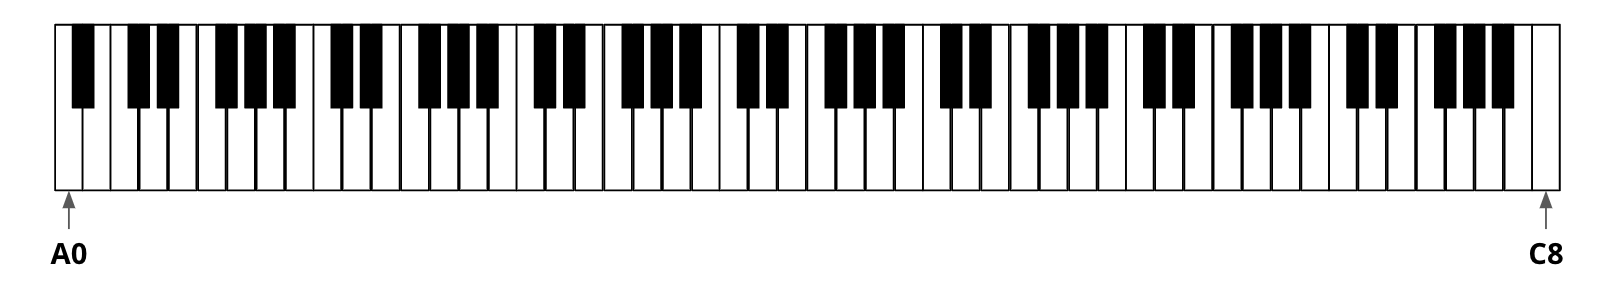
\includegraphics[width=0.9\columnwidth]{figure/piano.png}
\caption{88鍵のピアノの鍵盤}
\label{fig:piano}
\end{figure}

\section{提案モデル}
\label{sec:proposed}

本研究では、Pix2pix~\cite{pix2pix}を元に生成モデルと識別のいずれにも条件として変換元の音を入力することで音色の変換を行うGANを提案モデルとして作成した~(\prettyref{fig:pr_model})~。また、このモデルでは決定論的に音を生成するために生成モデルの入力にノイズを使用していない。

そして、本節の図の灰色の箱は複数のチャンネルを持つ特徴量マップである。箱の上側にチャンネル数を示し、箱の左側に特徴量マップとなる一次元配列の長さを示す。また、ネットワーク構造の下にそれぞれの矢印の操作の内容を示す。ConvolutionとDeconvolutionについては~(カーネルサイズ、パディング数、ストライド幅)~としてそれぞれの値を示し、LeakeyReLUについては負の実数の定義域での一次関数の傾きの値を示す。

%ここで改ページ
\clearpage

\begin{figure}[t]
\centering
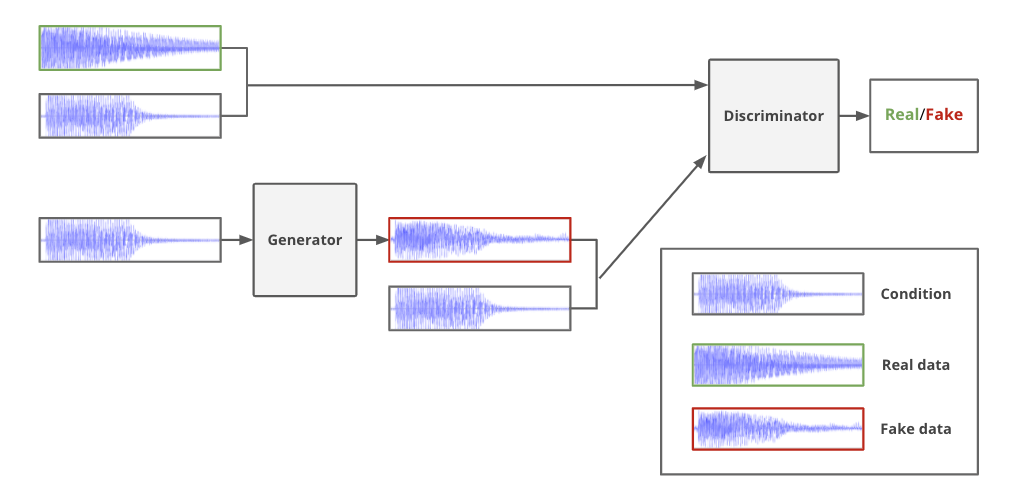
\includegraphics[width=0.8\columnwidth]{figure/pr_model.png}
\caption[本研究の提案モデル]{提案モデル}
\label{fig:pr_model}
\end{figure}

\subsection{生成モデル}

生成モデルには1つのスキップコネクションを持つEncoder-Decoder型のネットワークを用いた。また、入力は条件となる変換元の音波である~(\prettyref{fig:pr_gen})~。

\subsection{識別モデル}

識別モデルには一般的なCNNを用いた。また、出力は最終層の特徴量マップの平均値である~(\prettyref{fig:pr_dis})~。

\begin{figure}[b]
\centering
\begin{minipage}[b]{0.48\columnwidth}
\centering
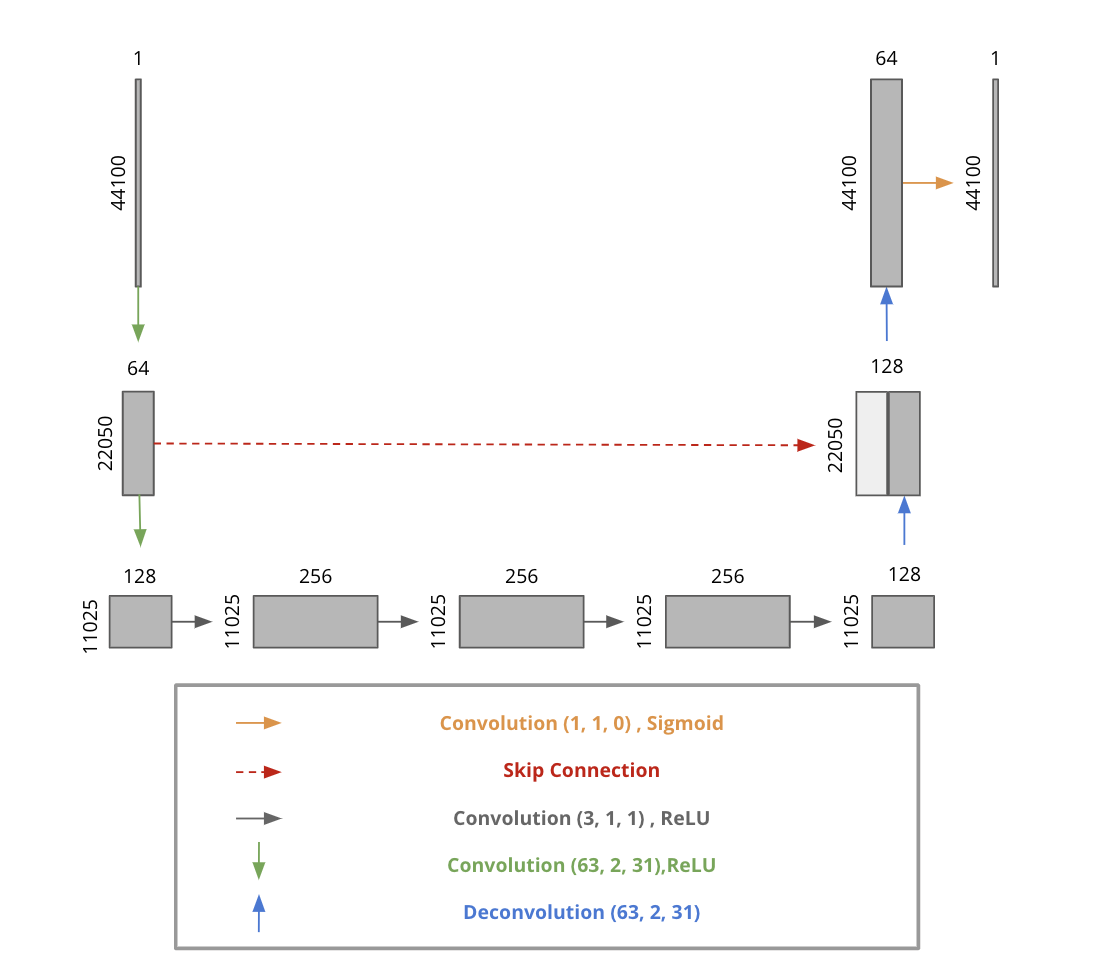
\includegraphics[width=0.8\columnwidth]{figure/pr_generator.png}
\subcaption[本研究の生成モデル]{生成モデルのネットワーク}
\label{fig:pr_gen}
\end{minipage}
\begin{minipage}[b]{0.48\columnwidth}
\centering
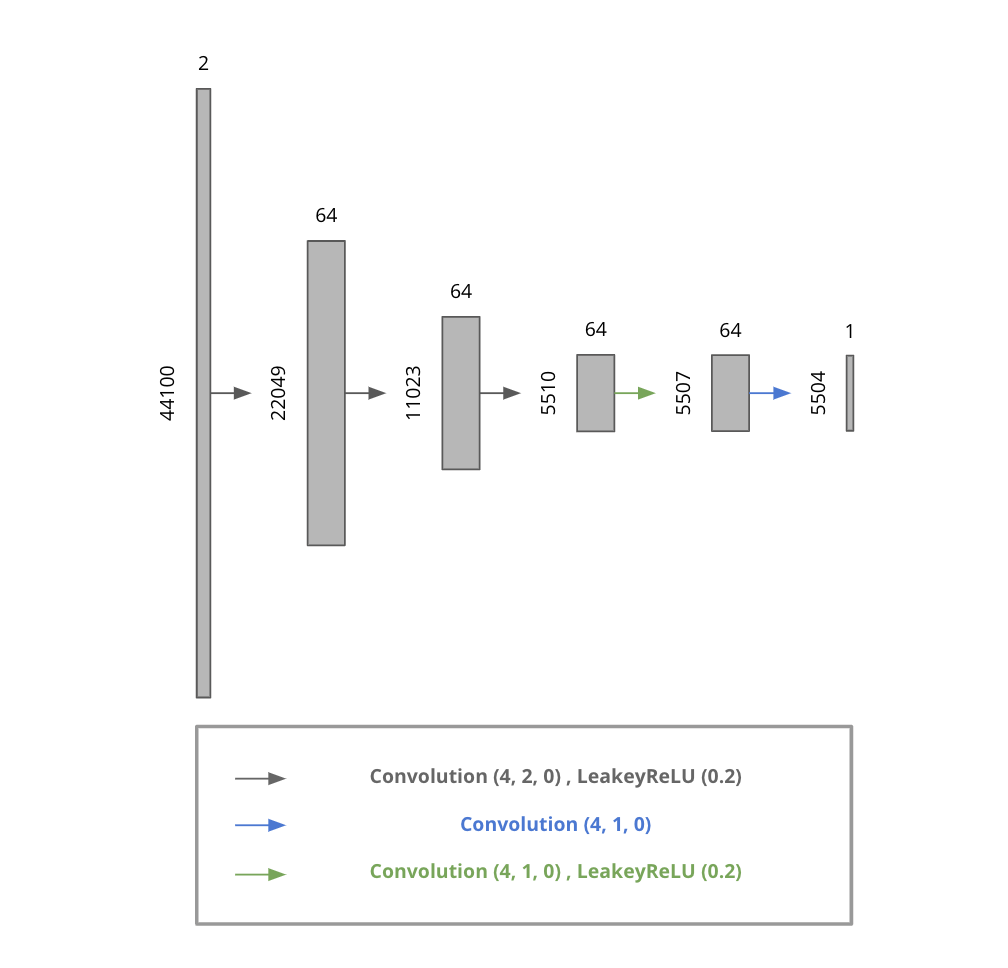
\includegraphics[width=0.8\columnwidth]{figure/pr_discriminator.png}
\subcaption[本研究の識別モデル]{識別モデルのネットワーク}
\label{fig:pr_dis}
\end{minipage}
\caption[本研究の生成モデルと識別モデル]{図は~\cite{u-net}のFigure~1を参考に作成した。}
\end{figure}

%ここで改ページ
\clearpage

\section{実験方法}

\prettyref{sec:proposed}の提案モデルを用いてギターからハープへの単音の変換の実験を行った。また、最適化アルゴリズムとして用いたAdam~\cite{Adam}のハイパーパラメータを\prettyref{app:params}に示す。

\subsection{提案モデルの表現力の評価実験}

提案モデルの表現力を評価する実験を行った。具体的には、用意した88音を学習データと評価データのいずれでも使用し、同じ高さの音の間での変換の実験を行った。

\subsection{提案モデルの汎化能力の評価実験}

単色の音色変換であっても任意の高さと大きさの音を学習データとして用意するのは不可能であるため、提案モデルの汎化能力を評価する必要がある。ここでは、88音のうち3/4を学習データ、1/4を評価データとする4分割交差検定により実験を行った。また、データセットの分割方法は\prettyref{app:split}に示す。

\subsection{評価方法}

生成した音を音波の波形の観察と音の聴き取りにより考察することで評価した。また、生成モデルの出力が音の高さ及び音の大きさを保持したまま変換先のハープの音の音色に変換できているかという観点から評価を行った。

\subsection{データ拡張}

各エポックの任意の学習データの振幅を無作為化することでデータ拡張を行った。具体的には、学習前に乱数のシードを固定した後に一様乱数により$0.3\sim1.0$の乱数を生成した。また、これにより88音と小さいサイズのデータセットへの過学習を防ぐことを期待した。

%ここで改ページ
\clearpage

\section{実験結果}
\label{sec:result}

実験結果の考察を本節では行う。また、実験結果に記載する波形の図は三つの波形を上から並べている。これらは上から順に、変換元のギターの波形、生成モデルの出力波形、変換先のハープの波形、である。そして、本節では一部の音波のみを記載しているが、\prettyref{app:result}に他の音波の波形を記載している。

\subsection{概要:提案モデルの表現力の評価実験}

提案モデルの表現力の評価実験を行ったところ、実験結果は二つに大別された。

\subsubsection{ハープの音を表現できた場合}

88音のうち86音はハープの音を表現することができた。~(\prettyref{fig:88_88_good1})~。また、特にC4からD5$\sharp$は目標のハープの音に極めて近い音を生成することができた~(\prettyref{fig:88_88_good2})~。これらの音は上音が少ないため、他の音と比べて表現が容易であったと推察される。

\begin{figure}[b]
\centering
\begin{minipage}{0.48\columnwidth}
\centering
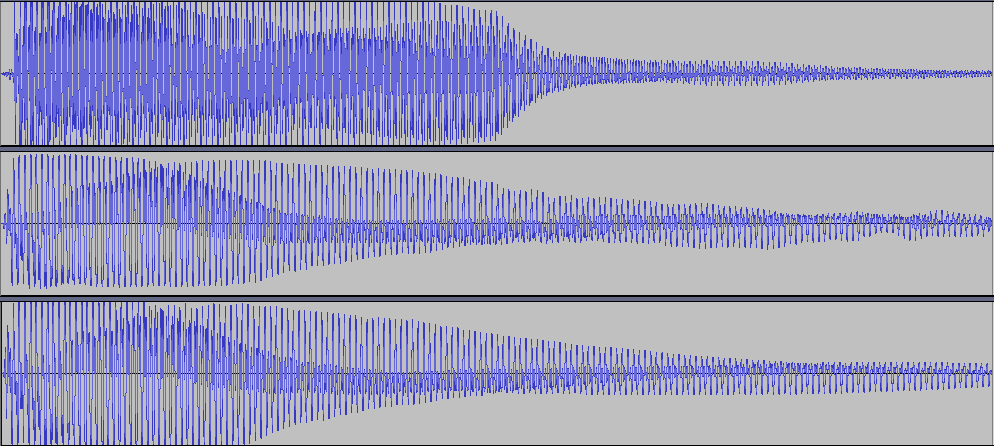
\includegraphics[width=0.9\columnwidth]{figure/88_88/f3.png}
\caption[F3の音波]{F3の0.800秒から1.000秒までの音波}
\label{fig:88_88_good1}
\end{minipage}
\begin{minipage}{0.48\columnwidth}
\centering
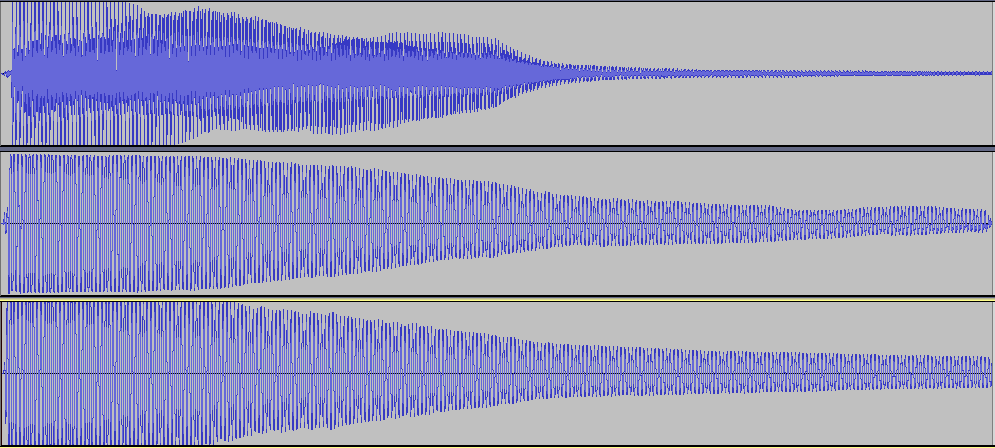
\includegraphics[width=0.9\columnwidth]{figure/88_88/c4.png}
\caption[C4の音波]{C4の0.200秒から0.300秒までの音波}
\label{fig:88_88_good2}
\end{minipage}
\end{figure}

%ここで改ページ
\clearpage

\subsubsection{ハープの音を表現できなかった場合}

D7$\sharp$とE7の2音は音の高さは維持できたものの、ハープの音を十分に表現できなかった~(\prettyref{fig:88_88_bad1}と\prettyref{fig:88_88_bad2})~。いずれの音についてもハープの音波の振動が安定しておらず、この不安定さを表現することはできなかった。また、他の高音においても振動が不安定なものが見られたため、高音において安定したデータセットをハープで生成するのが難しいと推察される。

\begin{figure}[b]
\centering
\begin{minipage}{0.48\columnwidth}
\centering
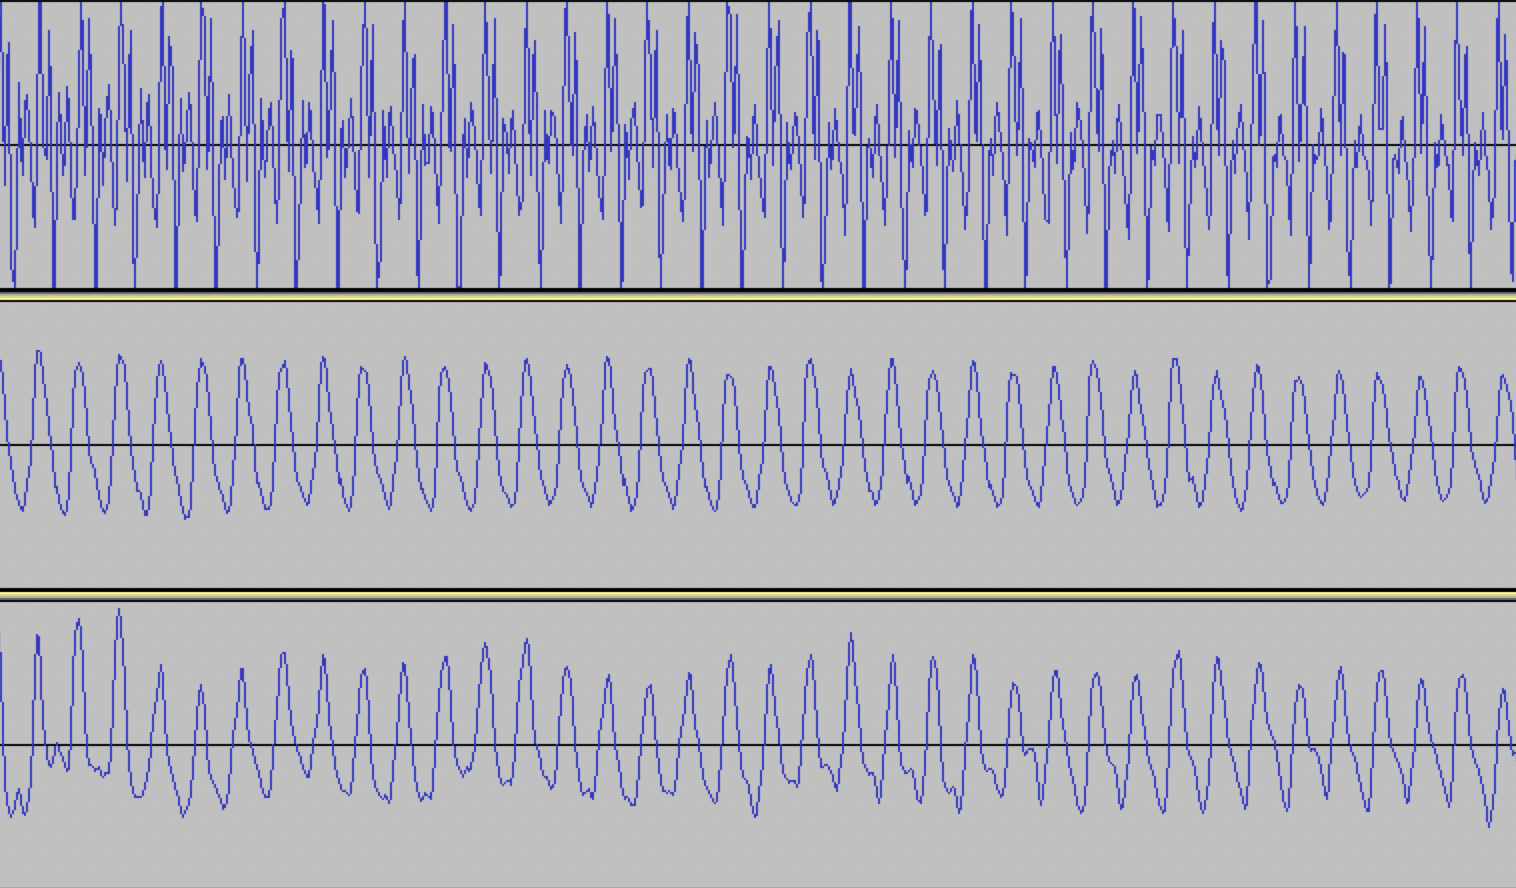
\includegraphics[width=0.9\columnwidth]{figure/88_88_det/d7s_0550_0700.png}
\caption[D7$\sharp$の音波]{D7$\sharp$の0.055秒から0.070秒までの音波}
\label{fig:88_88_bad1}
\end{minipage}
\begin{minipage}{0.48\columnwidth}
\centering
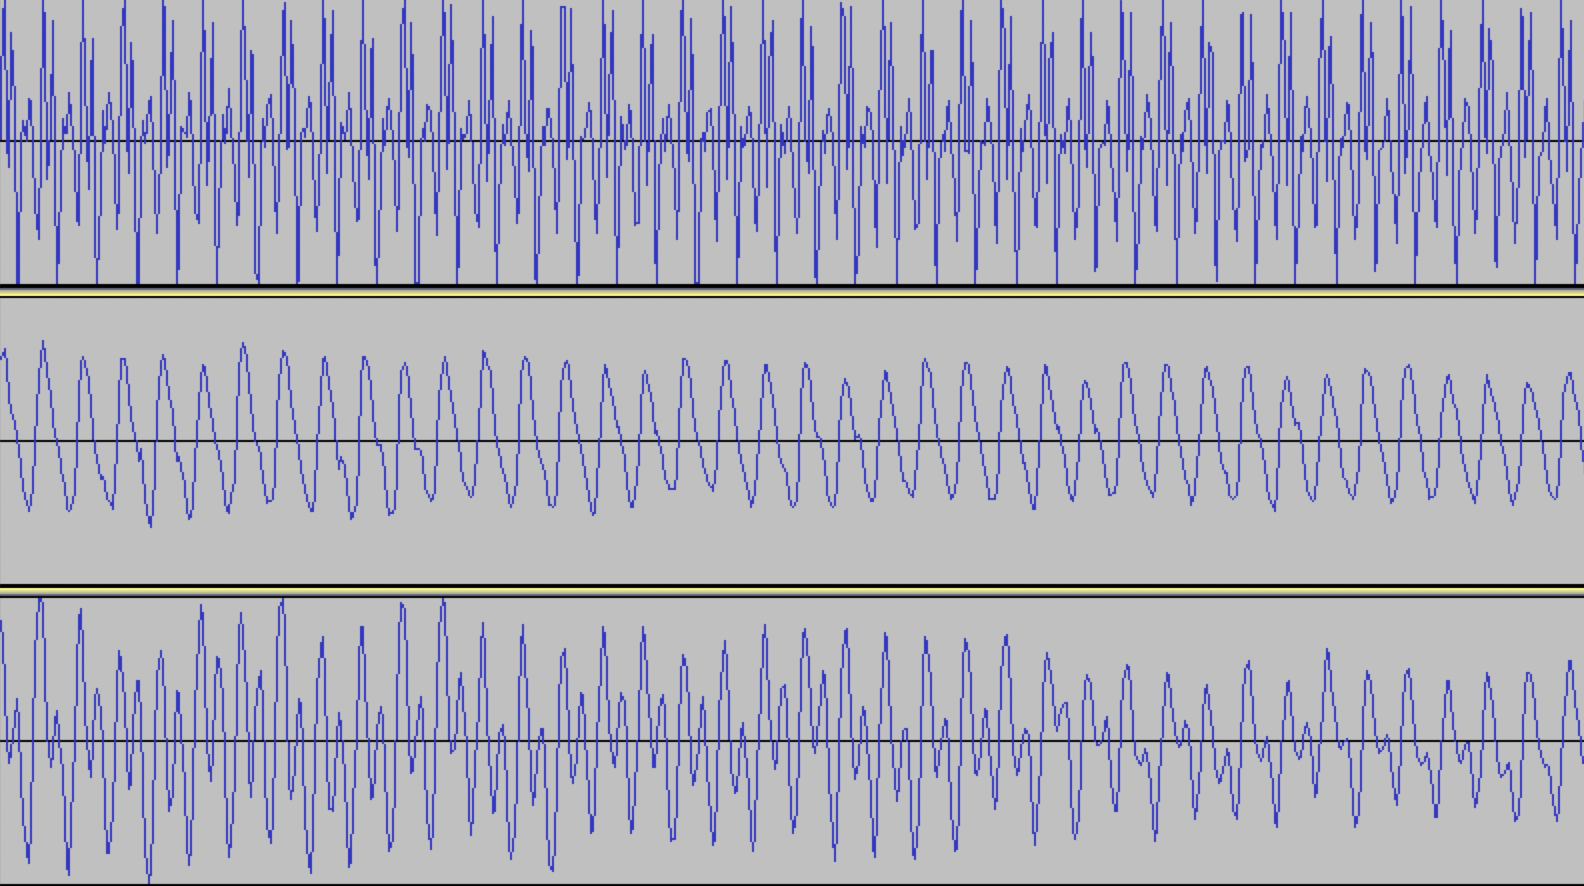
\includegraphics[width=0.9\columnwidth]{figure/88_88_det/e7_0550_0700.png}
\caption[E7の音波]{E7の0.055秒から0.070秒までの音波}
\label{fig:88_88_bad2}
\end{minipage}
\end{figure}

\subsection{概要:提案モデルの汎化能力の評価実験}

提案モデルの汎化能力の評価実験を行ったところ、実験結果は三つに大別された。

\subsubsection{ハープの音を表現できた場合}

D4,D4$\sharp$,G4,F5,F5$\sharp$の5音はハープの音を表現することができた~(\prettyref{fig:66_22_near})~。これらの高さの音では、提案モデルの表現力の評価実験の際にも特に綺麗なハープの音を表現できており、上音が少ないほど表現が容易であるという推察を示していると思われる。

\subsubsection{ハープの音を表現できず音の高さも維持できなかった場合}

C7,D7$\sharp$,E7,F7$\sharp$,G7,G7$\sharp$,A7,B7,C8の9音は音の高さも維持することができず、騒音が生成された~(\prettyref{fig:66_22_bad4})~。これらの高さの音では提案モデルの表現力の評価実験の際にもハープの音を表現できておらず、やはり高音域における安定したデータセットの作成は難しいと考えられる。また、高音域では周波数が高くノイズの影響が大きく出たとも考えられる。

\begin{figure}[b]
\centering
\begin{minipage}{0.48\columnwidth}
\centering
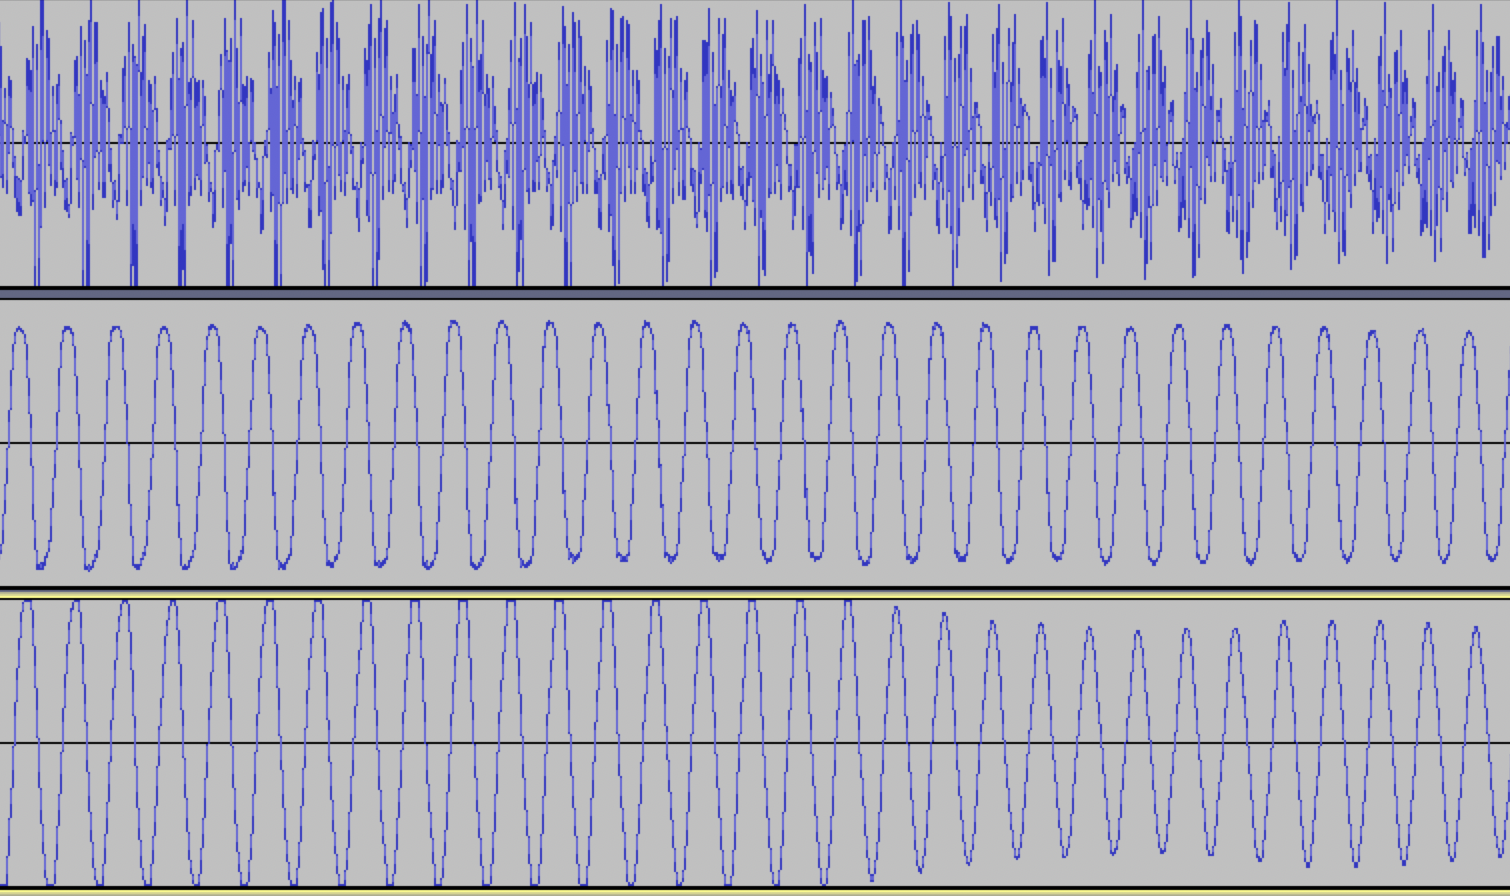
\includegraphics[width=0.85\columnwidth]{figure/66_22_det/d4s_0100_0200.png}
\caption[D4$\sharp$の音波]{D4$\sharp$の0.100秒から0.200秒までの音波}
\label{fig:66_22_near}
\end{minipage}
\begin{minipage}{0.48\columnwidth}
\centering
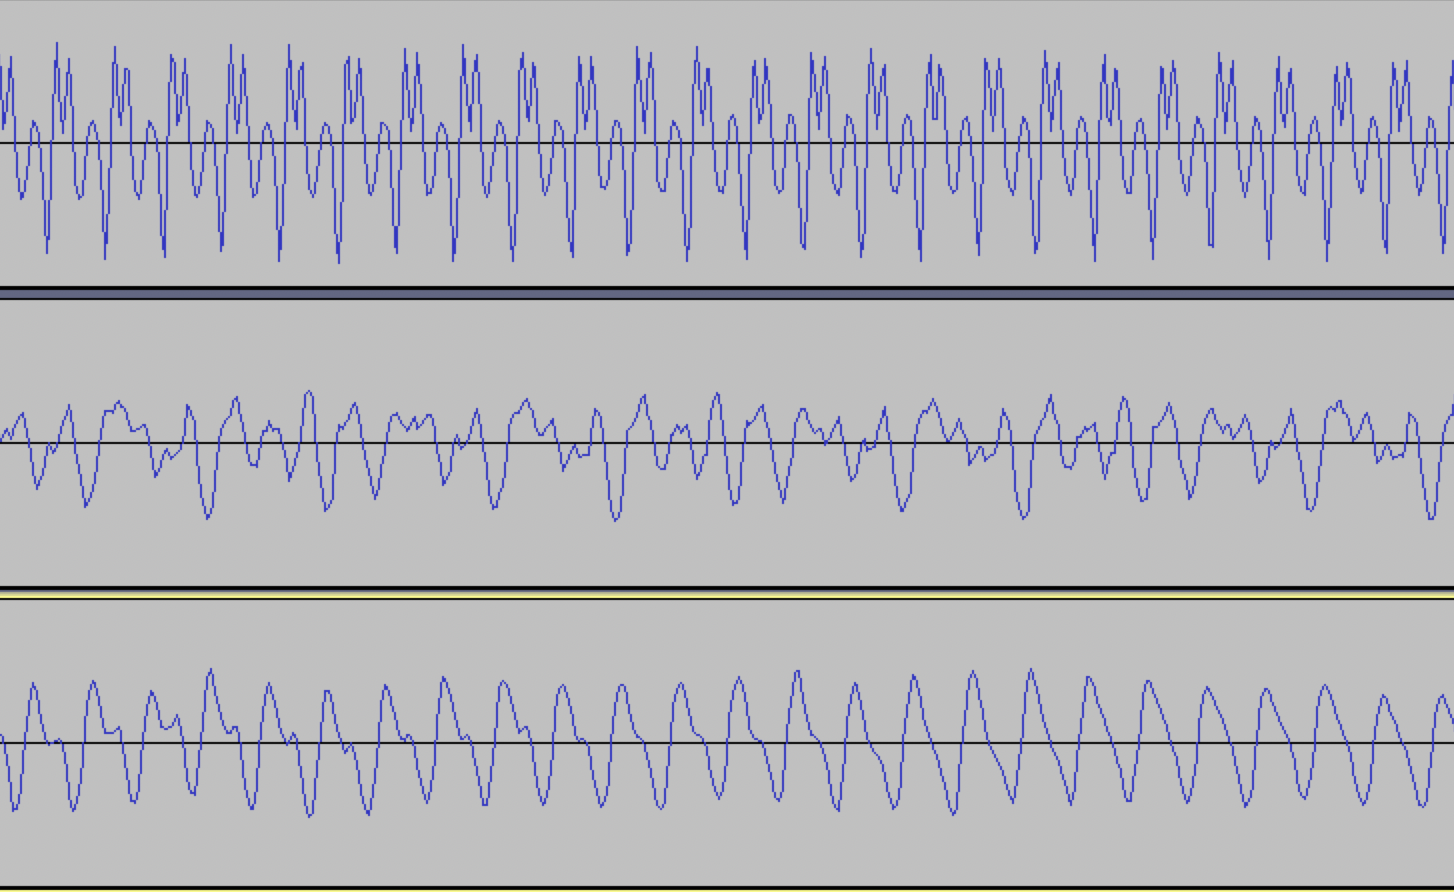
\includegraphics[width=0.85\columnwidth]{figure/66_22_det/d7s_0100_0110.png}
\caption[D7$\sharp$の音波]{D7$\sharp$の0.1700秒から0.110秒までの音波}
\label{fig:66_22_bad4}
\end{minipage}
\end{figure}

%ここで改ページ
\clearpage

\subsubsection{ハープの音を表現できず音の高さを維持できた場合}

14音を除く74音については音の高さは維持できているもののハープの音を表現することができなかった~(\prettyref{fig:66_22_bad1}、\prettyref{fig:66_22_bad2})~。これらの音では、音波が安定した振動をせず上音の成分がハープよりも多い音波が多く観測された。また、これらの高さの音は提案モデルの表現力の評価実験の際には表現することができていたため、提案モデルの汎化能力の低さが明らかになった。

\begin{figure}[b]
\centering
\begin{minipage}{0.48\columnwidth}
\centering
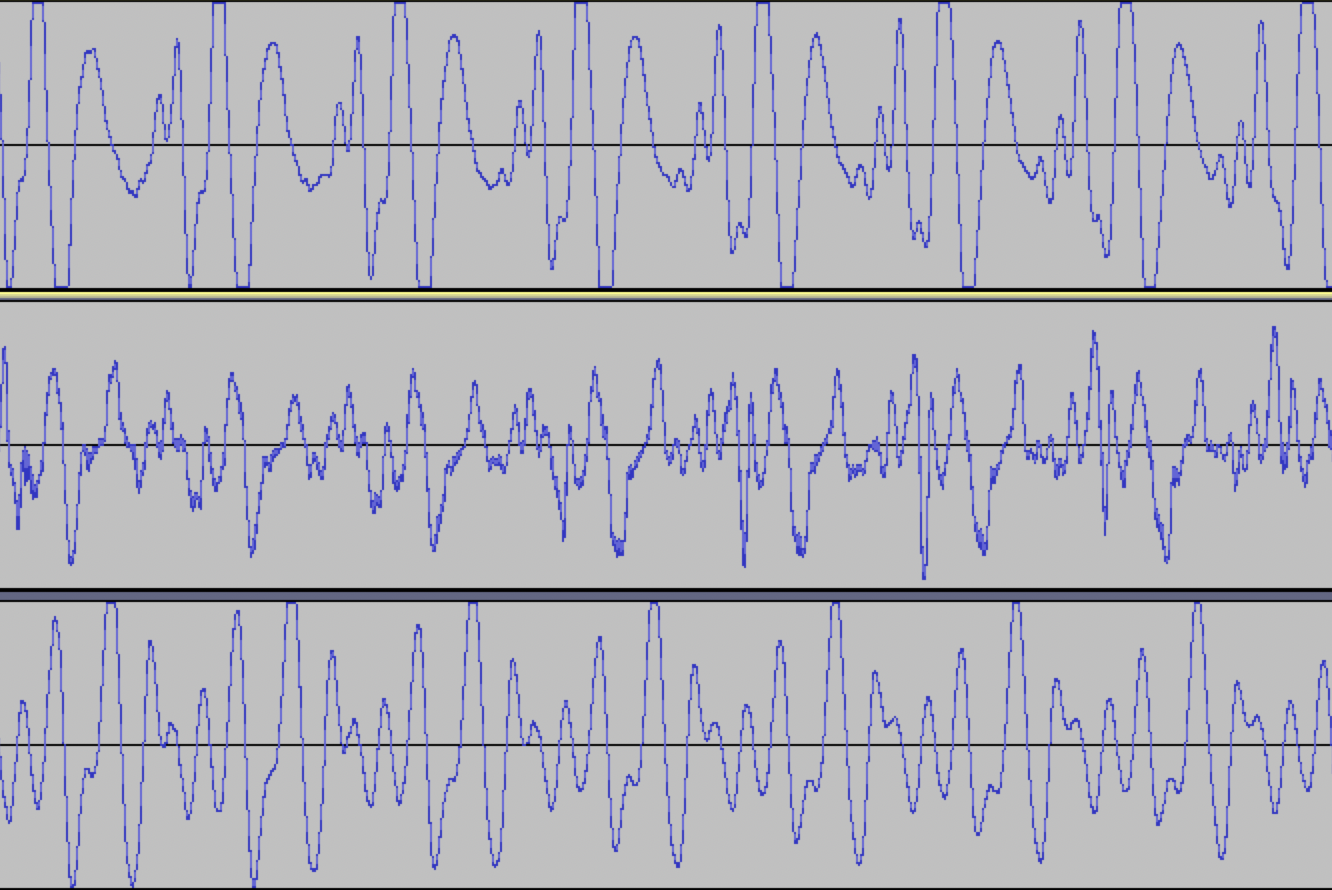
\includegraphics[width=0.75\columnwidth]{figure/66_22_det/d1_0300_0500.png}
\caption[D1の音波]{D1の0.300秒から0.500秒までの音波}
\label{fig:66_22_bad1}
\end{minipage}
\begin{minipage}{0.48\columnwidth}
\centering
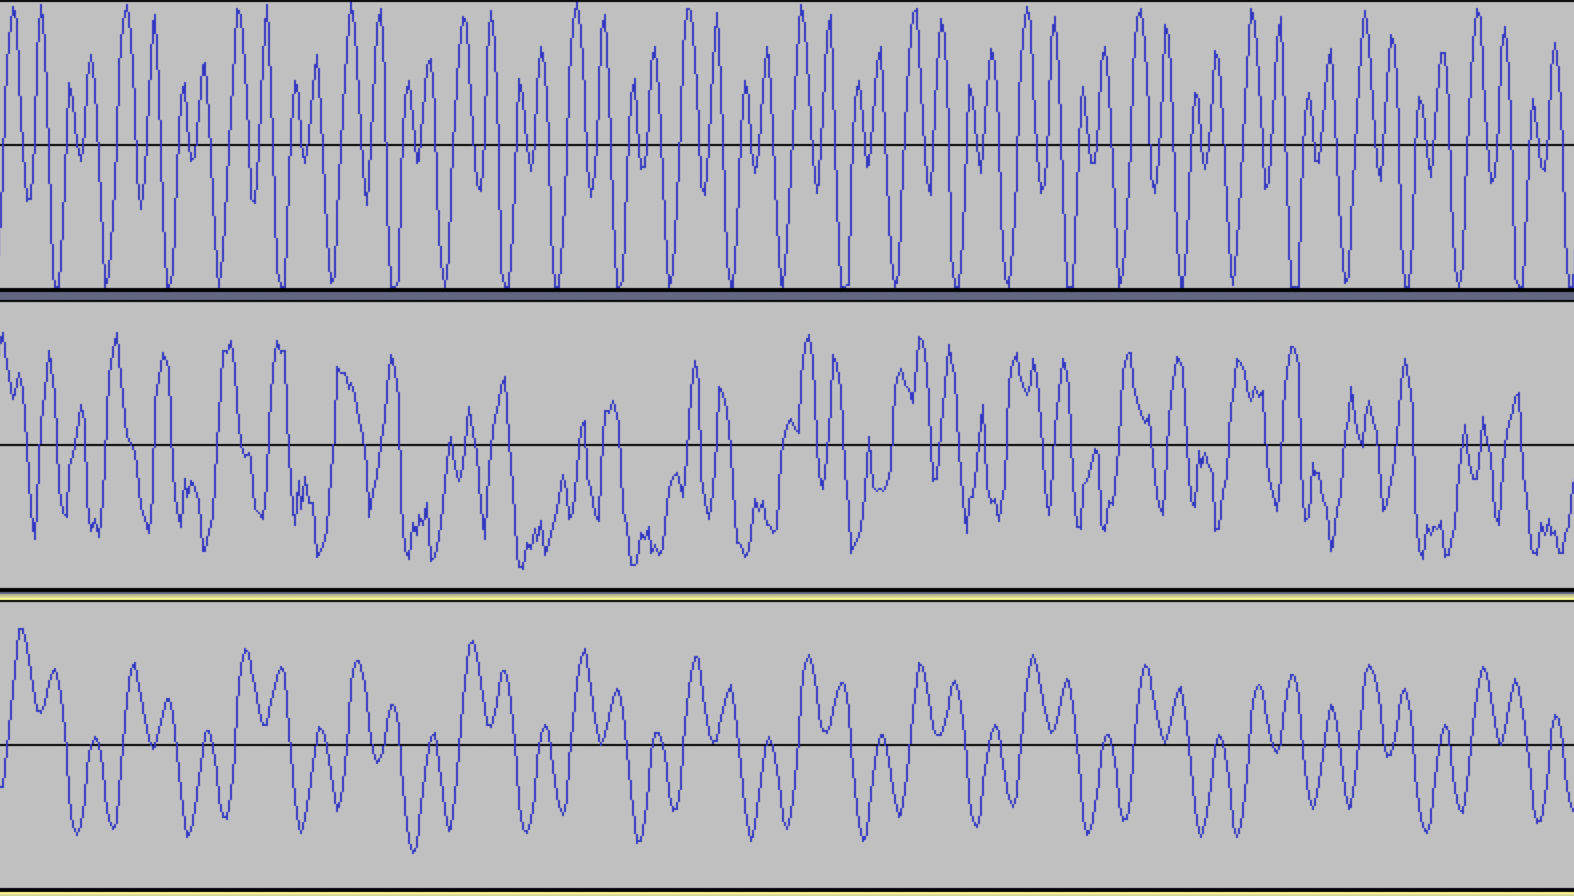
\includegraphics[width=0.85\columnwidth]{figure/66_22_det/f6_0070_0080.png}
\caption[F6の音波]{F6の0.070秒から0.080秒までの音波}
\label{fig:66_22_bad2}
\end{minipage}
\end{figure}

\subsection{課題}

実験結果から四つの課題が明らかになった。

\subsubsection{音の減衰の表現}

振動の減衰を表現できていない音がいくつかあった。これらの音のうち、E2以下の低音域ではハープとは全く異なる波形で減衰し~(\prettyref{fig:88_88_reduce1})~、A6以上の高音域ではほとんど振動が見られなかった~(\prettyref{fig:88_88_reduce2})~。また、提案モデルでは表現力が足りず微小な振動の学習が難しいためであると考えられる。

\begin{figure}[b]
\centering
\begin{minipage}{0.48\columnwidth}
\centering
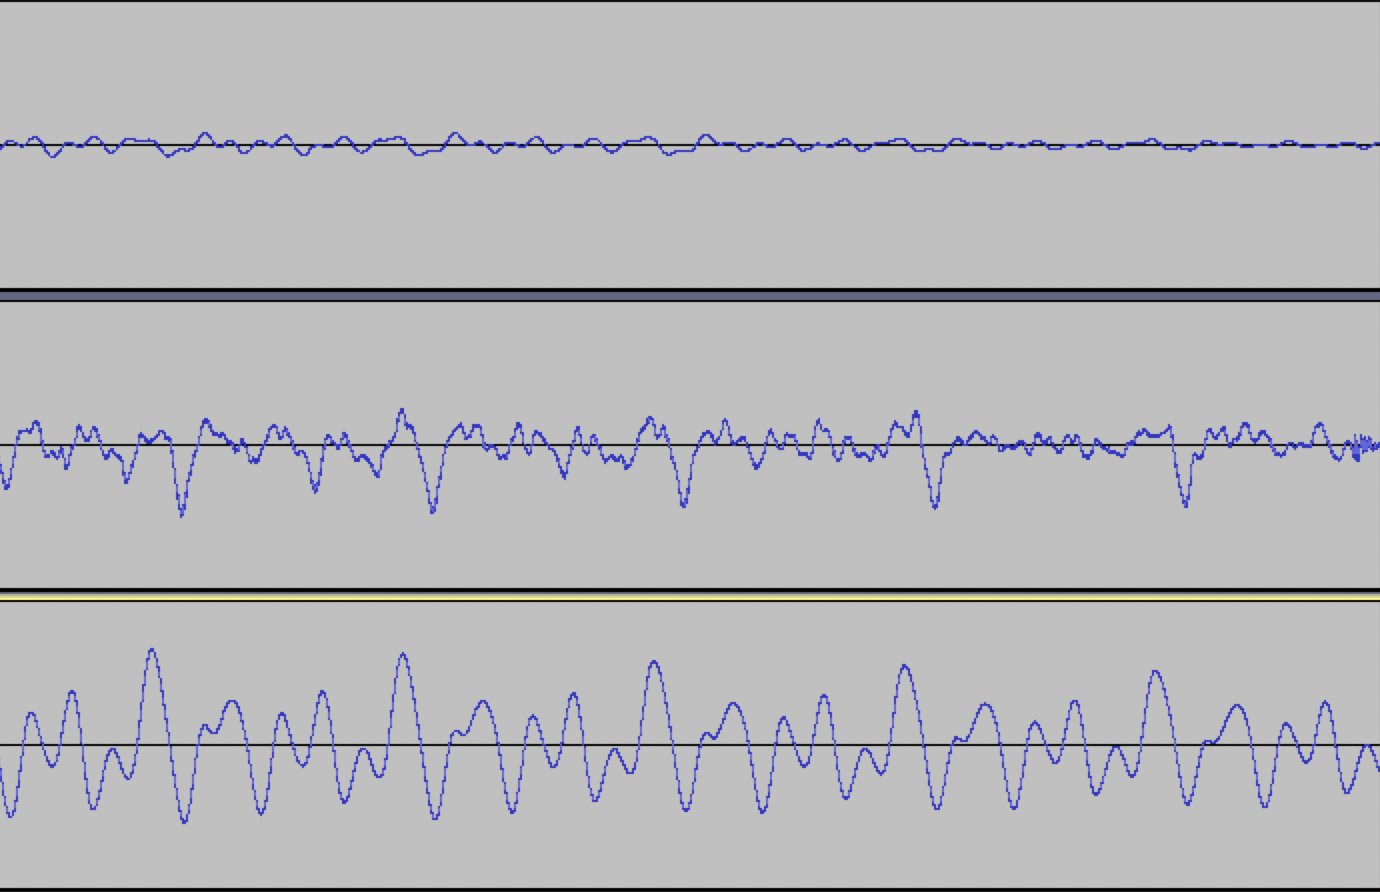
\includegraphics[width=0.85\columnwidth]{figure/88_88_det/a0_0800_1000.png}
\caption[A0の音波]{A0の0.800秒から1.000秒までの音波}
\label{fig:88_88_reduce1}
\end{minipage}
\begin{minipage}{0.48\columnwidth}
\centering
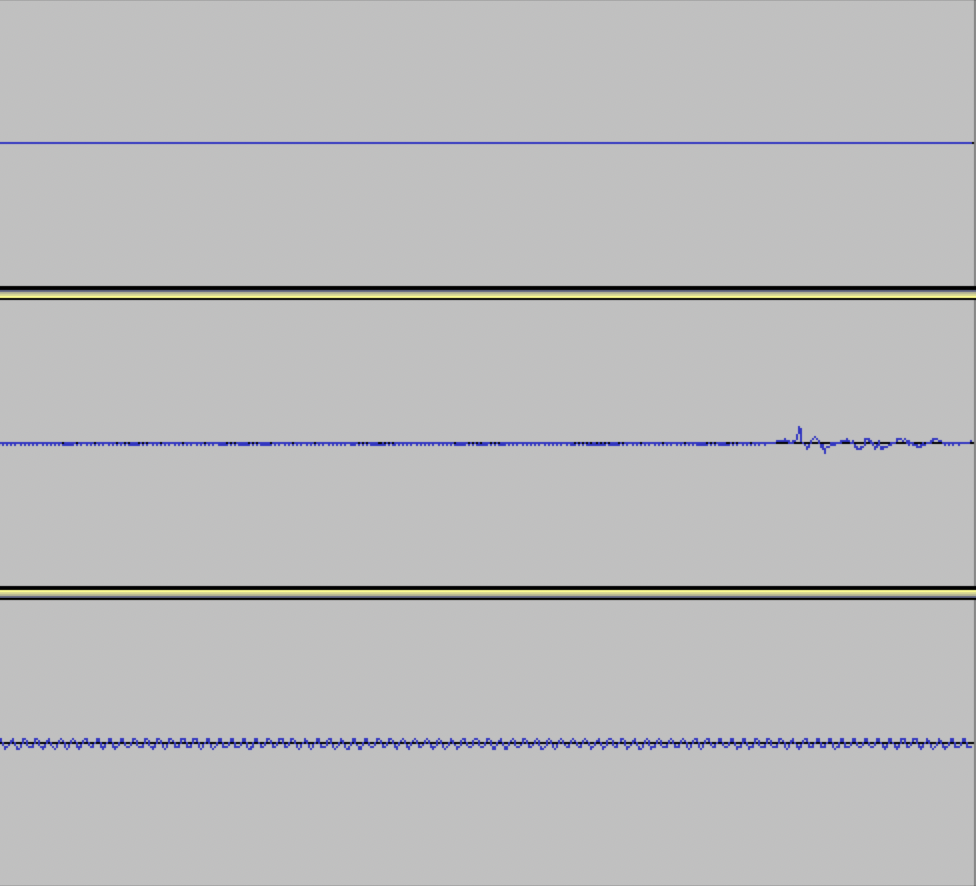
\includegraphics[width=0.75\columnwidth]{figure/88_88_det/b7_0980_1000.png}
\caption[B7の音波]{B7の0.980秒から1.000秒までの音波}
\label{fig:88_88_reduce2}
\end{minipage}
\end{figure}

%ここで改ページ
\clearpage

\subsubsection{音の大きさの維持}

部分的に大きさを維持できていない音がいくつかあった。\prettyref{fig:88_88_amp}では、波形の前半において生成波形の振幅が小さいことがわかる。原因は振幅をランダムに小さくしたことにあると考えられ、学習の初段階では振幅を固定しておくことや振幅の大きさを別で調整するなどの工夫が必要であると考えられる。
    
\subsubsection{音波の滑らかさの表現}

ノイズまじりの音がいくつかあった。これらの音を詳細に観察すると、生成された音波では滑らかさを表現できていないことがわかった~(\prettyref{fig:88_88_smooth})~。音波を滑らかにするような加工を生成後に加えるなどの工夫が必要であると考えられる。

\begin{figure}[b]
\centering
\begin{minipage}{0.48\columnwidth}
\centering
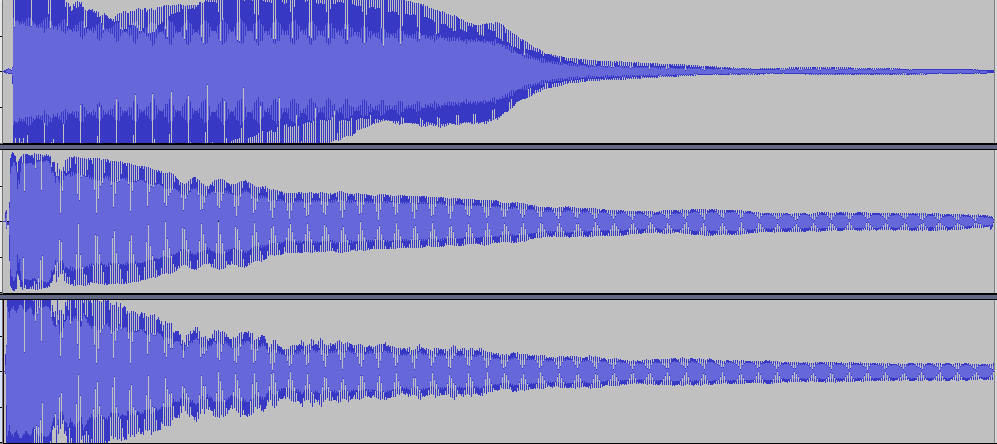
\includegraphics[width=0.85\columnwidth]{figure/88_88/c5.png}
\caption[C5の音波]{C5の0.000秒から1.000秒までの音波}
\label{fig:88_88_amp}
\end{minipage}
\begin{minipage}{0.48\columnwidth}
\centering
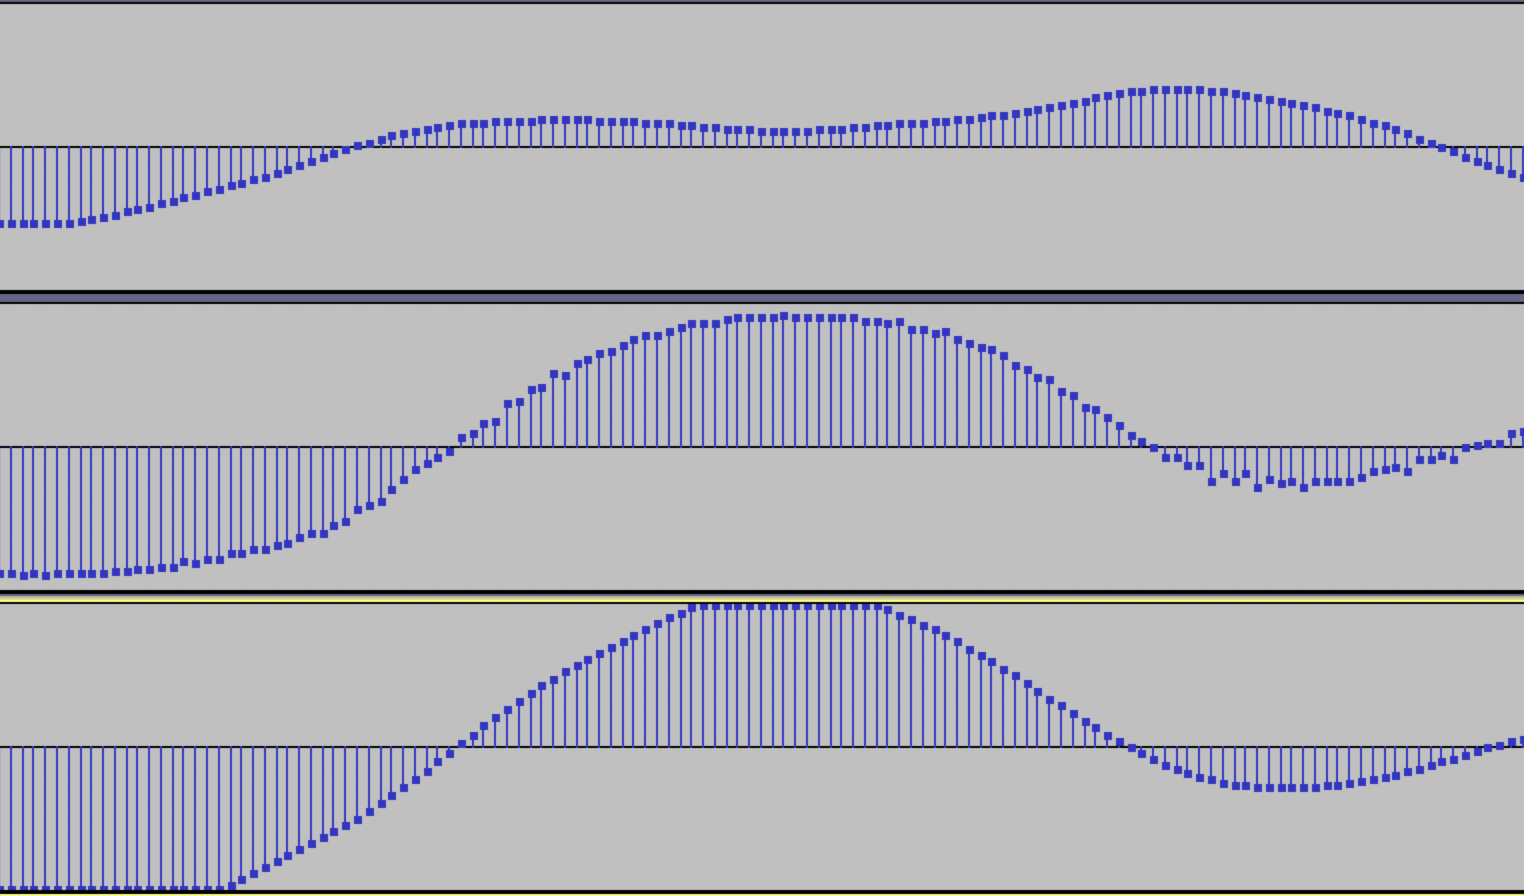
\includegraphics[width=0.75\columnwidth]{figure/88_88_det/d2s_0100_0103.png}
\caption[D2$\sharp$の音波]{D2$\sharp$の0.100秒から0.103秒までの音波}
\label{fig:88_88_smooth}
\end{minipage}
\end{figure}

\subsubsection{データセットの不安定さ}

ここまでの三つは提案モデルの改善により解消されると考えられるが、問題のあるデータセットも一部に存在した。一つの問題点は高音において振動が不安定になることであり、ここまでで述べた。もう一つの問題点は音の鳴り出しでの振動が不安定であるという点である。具体的には、\prettyref{fig:88_88_lag1}のようにギターの音の鳴り出しの遅延の方がハープより大きい場合や\prettyref{fig:88_88_lag2}のように周期的な音になるまでに遅延があるために不規則な振動となる場合などがあった。

\begin{figure}[b]
\centering
\begin{minipage}{0.48\columnwidth}
\centering
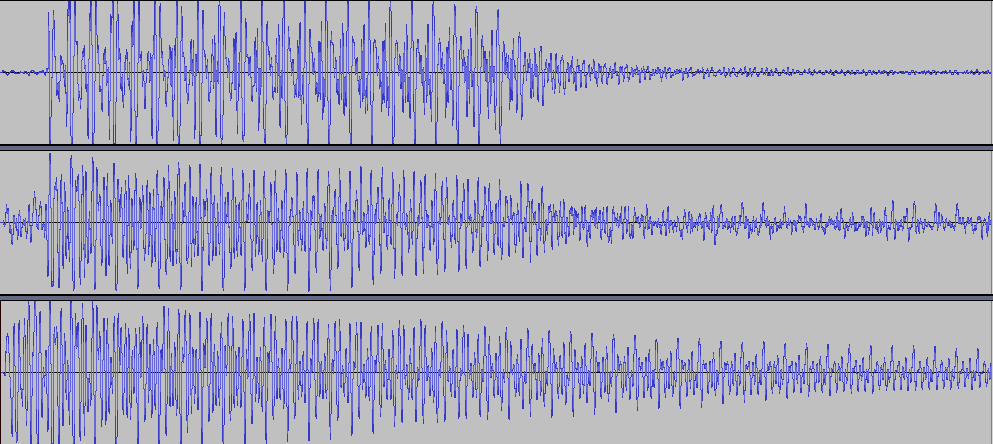
\includegraphics[width=0.9\columnwidth]{figure/88_88/f1s.png}
\caption[F1$\sharp$の音波]{F1$\sharp$の0.000秒から1.000秒までの音波}
\label{fig:88_88_lag1}
\end{minipage}
\begin{minipage}{0.48\columnwidth}
\centering
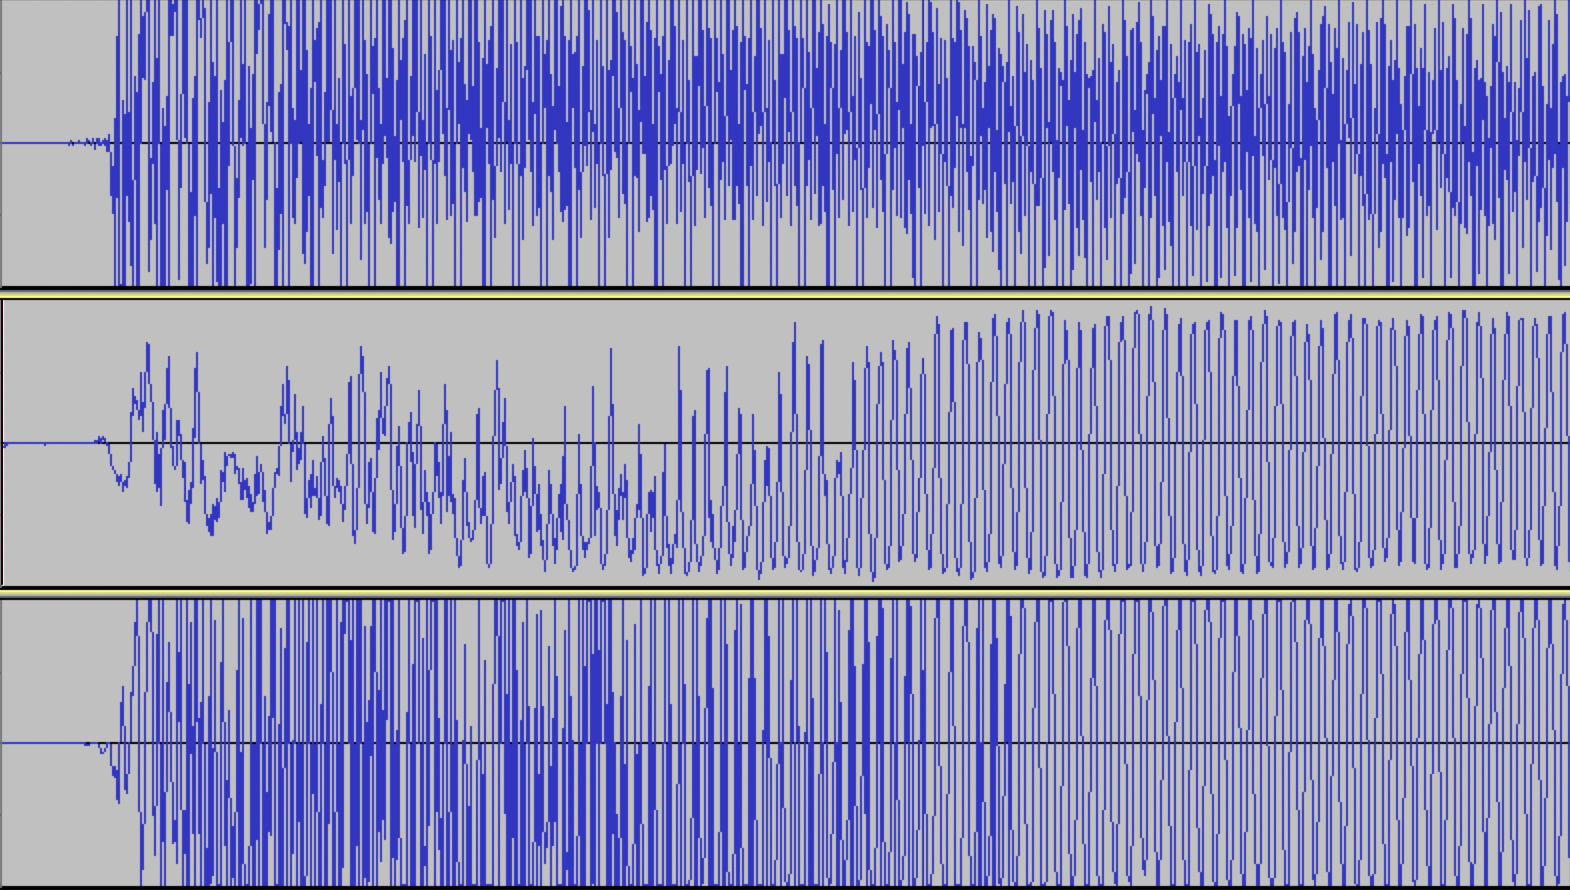
\includegraphics[width=0.75\columnwidth]{figure/88_88_det/a7_0_0030.png}
\caption[A7の音波]{A7の0.000秒から0.030秒までの音波}
\label{fig:88_88_lag2}
\end{minipage}
\end{figure}

%まとめ
%やったこと、やってないことを書く
%実験で見つかった課題とかも
\chapter{まとめ}

ネットワーク変えれるのでは?
もっとランダムにできるのでは?
本研究では〇〇を確認することができた。以後は以下をやる。


バランス悪いデータセットの可能性
→バランス良くしたら

ハープからギターの方向
別の楽器との比較


二音のみの組み合わせでできるのか
前処理を工夫するか
フーリエ変換を用いてsin波に分解するか

本研究では波形の観察による考察を行ったが、より定量的な判定を行うには判定器の導入が必要であると考えられ、具体的には以下の二点での判定が必要である。

(1)音程が維持されているか

(2)変換されて音色が変換されているか

波形とスペクトログラム?

%謝辞
\chapter*{謝辞}

%参考文献
\bibliographystyle{junsrt}
\bibliography{reference}

%付録
%追加すべき事項
% - 実験結果の画像の添付
% - DDSP解説?
% - ? Adamの説明
\appendix

\chapter{Adam}
\label{cha:Adam}

Adamは勾配降下法の中で最も用いられるアルゴリズムであり、\prettyref{alg:Adam}に示す手順にしたがってパラメータの更新を行う。また、アルゴリズムの詳細については~\cite{Adam}を参考にされたい。

\begin{algorithm}[b]
\label{alg:Adam}
    \DontPrintSemicolon
    \SetKwInOut{KwHyParam}{HyperParameter}
    \SetKwInOut{KwParam}{Parameter}
    \SetKwInOut{KwObFunc}{Objective~Function}
    \KwHyParam{$\beta_1,\beta_2\in \interval[open left]{0}{1},\eta,\epsilon$}
    \KwObFunc{$f$}
    \KwParam{$\theta$}
    \setlength{\alignwidth}{0.2\columnwidth}
    \Init{
        $t \leftarrow 0$ \tcc*{Initialize~timestep}\;
        $\theta \leftarrow \theta_0$ \tcc*{Initialize~Parameter}\;
        $m_1,m_2 \leftarrow 0,0$ \tcc*{Initialize~moments}\;
    }
    \setlength{\alignwidth}{0.58\columnwidth}
    \Proc{
        \While{$\theta$ not converged}{
            $t \leftarrow t+1$ \tcc*{Update~timestep}\;
            $g \leftarrow \nabla _{\theta} f(\theta)$ \tcc*{Compute~gradient~of~$f(\theta)$}\;
            $m_1,m_2 \leftarrow \beta_1 \cdot m_1+(1-\beta_1) \cdot g,\beta_2 \cdot m_2+(1-\beta_2) \cdot (g \odot g)$ \tcc*{Update~biased~moments}\;
            $\hat{m_1},\hat{m_2} \leftarrow m_1/(1-\beta_1^t),m_2/(1-\beta_2^t)$ \tcc*{Update~bias-corrected~moments}\;
            $\theta \leftarrow \theta - \eta \cdot \hat{m_1}/(\sqrt{\hat{m_2}}+\epsilon)$ \tcc*{Update~Parameter}\;
        }
        \Return{$\theta$}\;
    }
\caption{Adamの疑似コード}
\end{algorithm}

\chapter{学習時のパラメータ}
\label{app:params}

提案モデルの学習時のパラメータの値を\prettyref{tab:params1}に示す。また、\prettyref{tab:params2}は\prettyref{alg:Adam}に示すハイパーパラメータの値である。

\begin{table}[h]
\centering
\begin{minipage}{0.49\columnwidth}
    \centering
        \begin{tabular}{lr}\toprule
            パラメータ & 値 \\ \midrule
            バッチサイズ & 1 \\ 
            エポック数 & 1000 \\ \bottomrule
        \end{tabular}
    \caption{}
    \label{tab:params1}
\end{minipage}
\begin{minipage}{0.49\columnwidth}
    \centering
        \begin{tabular}{lr}\toprule
            パラメータ & 値 \\ \midrule
            $\beta_1$ & 0.5 \\
            $\beta_2$ & 0.999 \\
            $\eta$ & 0.0002 \\ 
            $\epsilon$ & $10^{-8}$ \\ \bottomrule
        \end{tabular}
    \caption{}
    \label{tab:params2}
\end{minipage}
\end{table}

\chapter{データセットの分割}
\label{app:split}

22音ずつの4つのサブセットにデータセットを分割した~(\prettyref{fig:data_div})~。また、データセットの4分割は、88音をシャッフルして配列に格納した後に22音ずつ順に選ぶことで実装した。

\begin{figure}[h]
\centering
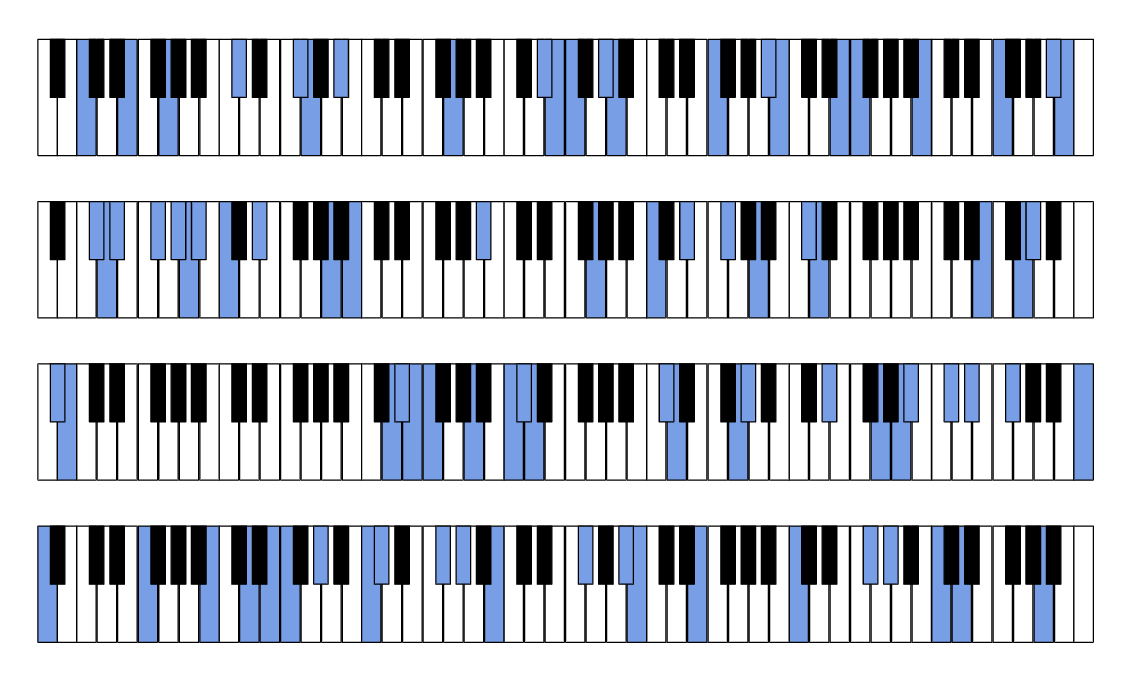
\includegraphics[width=\columnwidth]{figure/data_div.png}
\caption{データセットのサブセット}
\label{fig:data_div}
\end{figure}

\chapter{DDSP}
\label{app:DDSP}

\chapter{実験結果}
\label{app:result}

\prettyref{sec:result}に載せることのできなかった波形の図を本章に載せる

\section{提案モデルの表現力の評価実験}

提案モデルの評価実験を行ったところ、88音のうち87音については変換先のギターの音を表現できていると判断することができた。


\section{提案モデルの汎化能力の評価実験}

\end{document}